\documentclass[11pt,a4paper,notitlepage]{article}
\usepackage[latin1]{inputenc}
\usepackage{amsmath}
\usepackage{amsfonts}
\usepackage{amssymb}
\usepackage{graphicx}
\usepackage{epstopdf}
\usepackage[toc,page]{appendix}
\usepackage{fancyhdr}
\usepackage{titling}
\usepackage{pdfpages}
\usepackage{mcode}

\author{John Paul Alexander CID:00824301}
\title{M3N10: Final Project}


\pagestyle{fancy}
\lhead{John Paul Alexander}
\rhead{CID: 00824301}
\chead{M3N10: Final Project}


\begin{document}

\maketitle
\thispagestyle{empty}

\begin{abstract}
Extending cavity flow from a rectangular domain to an L shaped domain.\\

This is my own unaided work unless otherwise specified.\\

\end{abstract}

\tableofcontents

\newpage
%----------------------------------------------------------------------------------
\section{Advection}
%----------------------------------------------------------------------------------

The equation governing the motion of advection is the given below (\ref{Adv}) where $a_x$ and $a_y$ are parameters controlling the speed and direction of the solution.

\begin{equation} \label{Adv}
\frac{\partial q}{\partial t} + a_x \frac{\partial q}{\partial x} + a_y \frac{\partial q}{\partial y} = 0
\end{equation}

The code given to us can be easily extended by editing `SemiLagrAdvect.m' to accept rectangles of different sizes and calling the function twice giving the boundary conditions of the edge where it is so and an average of rows or columns of the previous solution where the boundary falls inside the L-shape. Then the two new partial solutions are stitched together to form the solution at the next step.

\begin{figure}[h]
\vspace{-10pt}
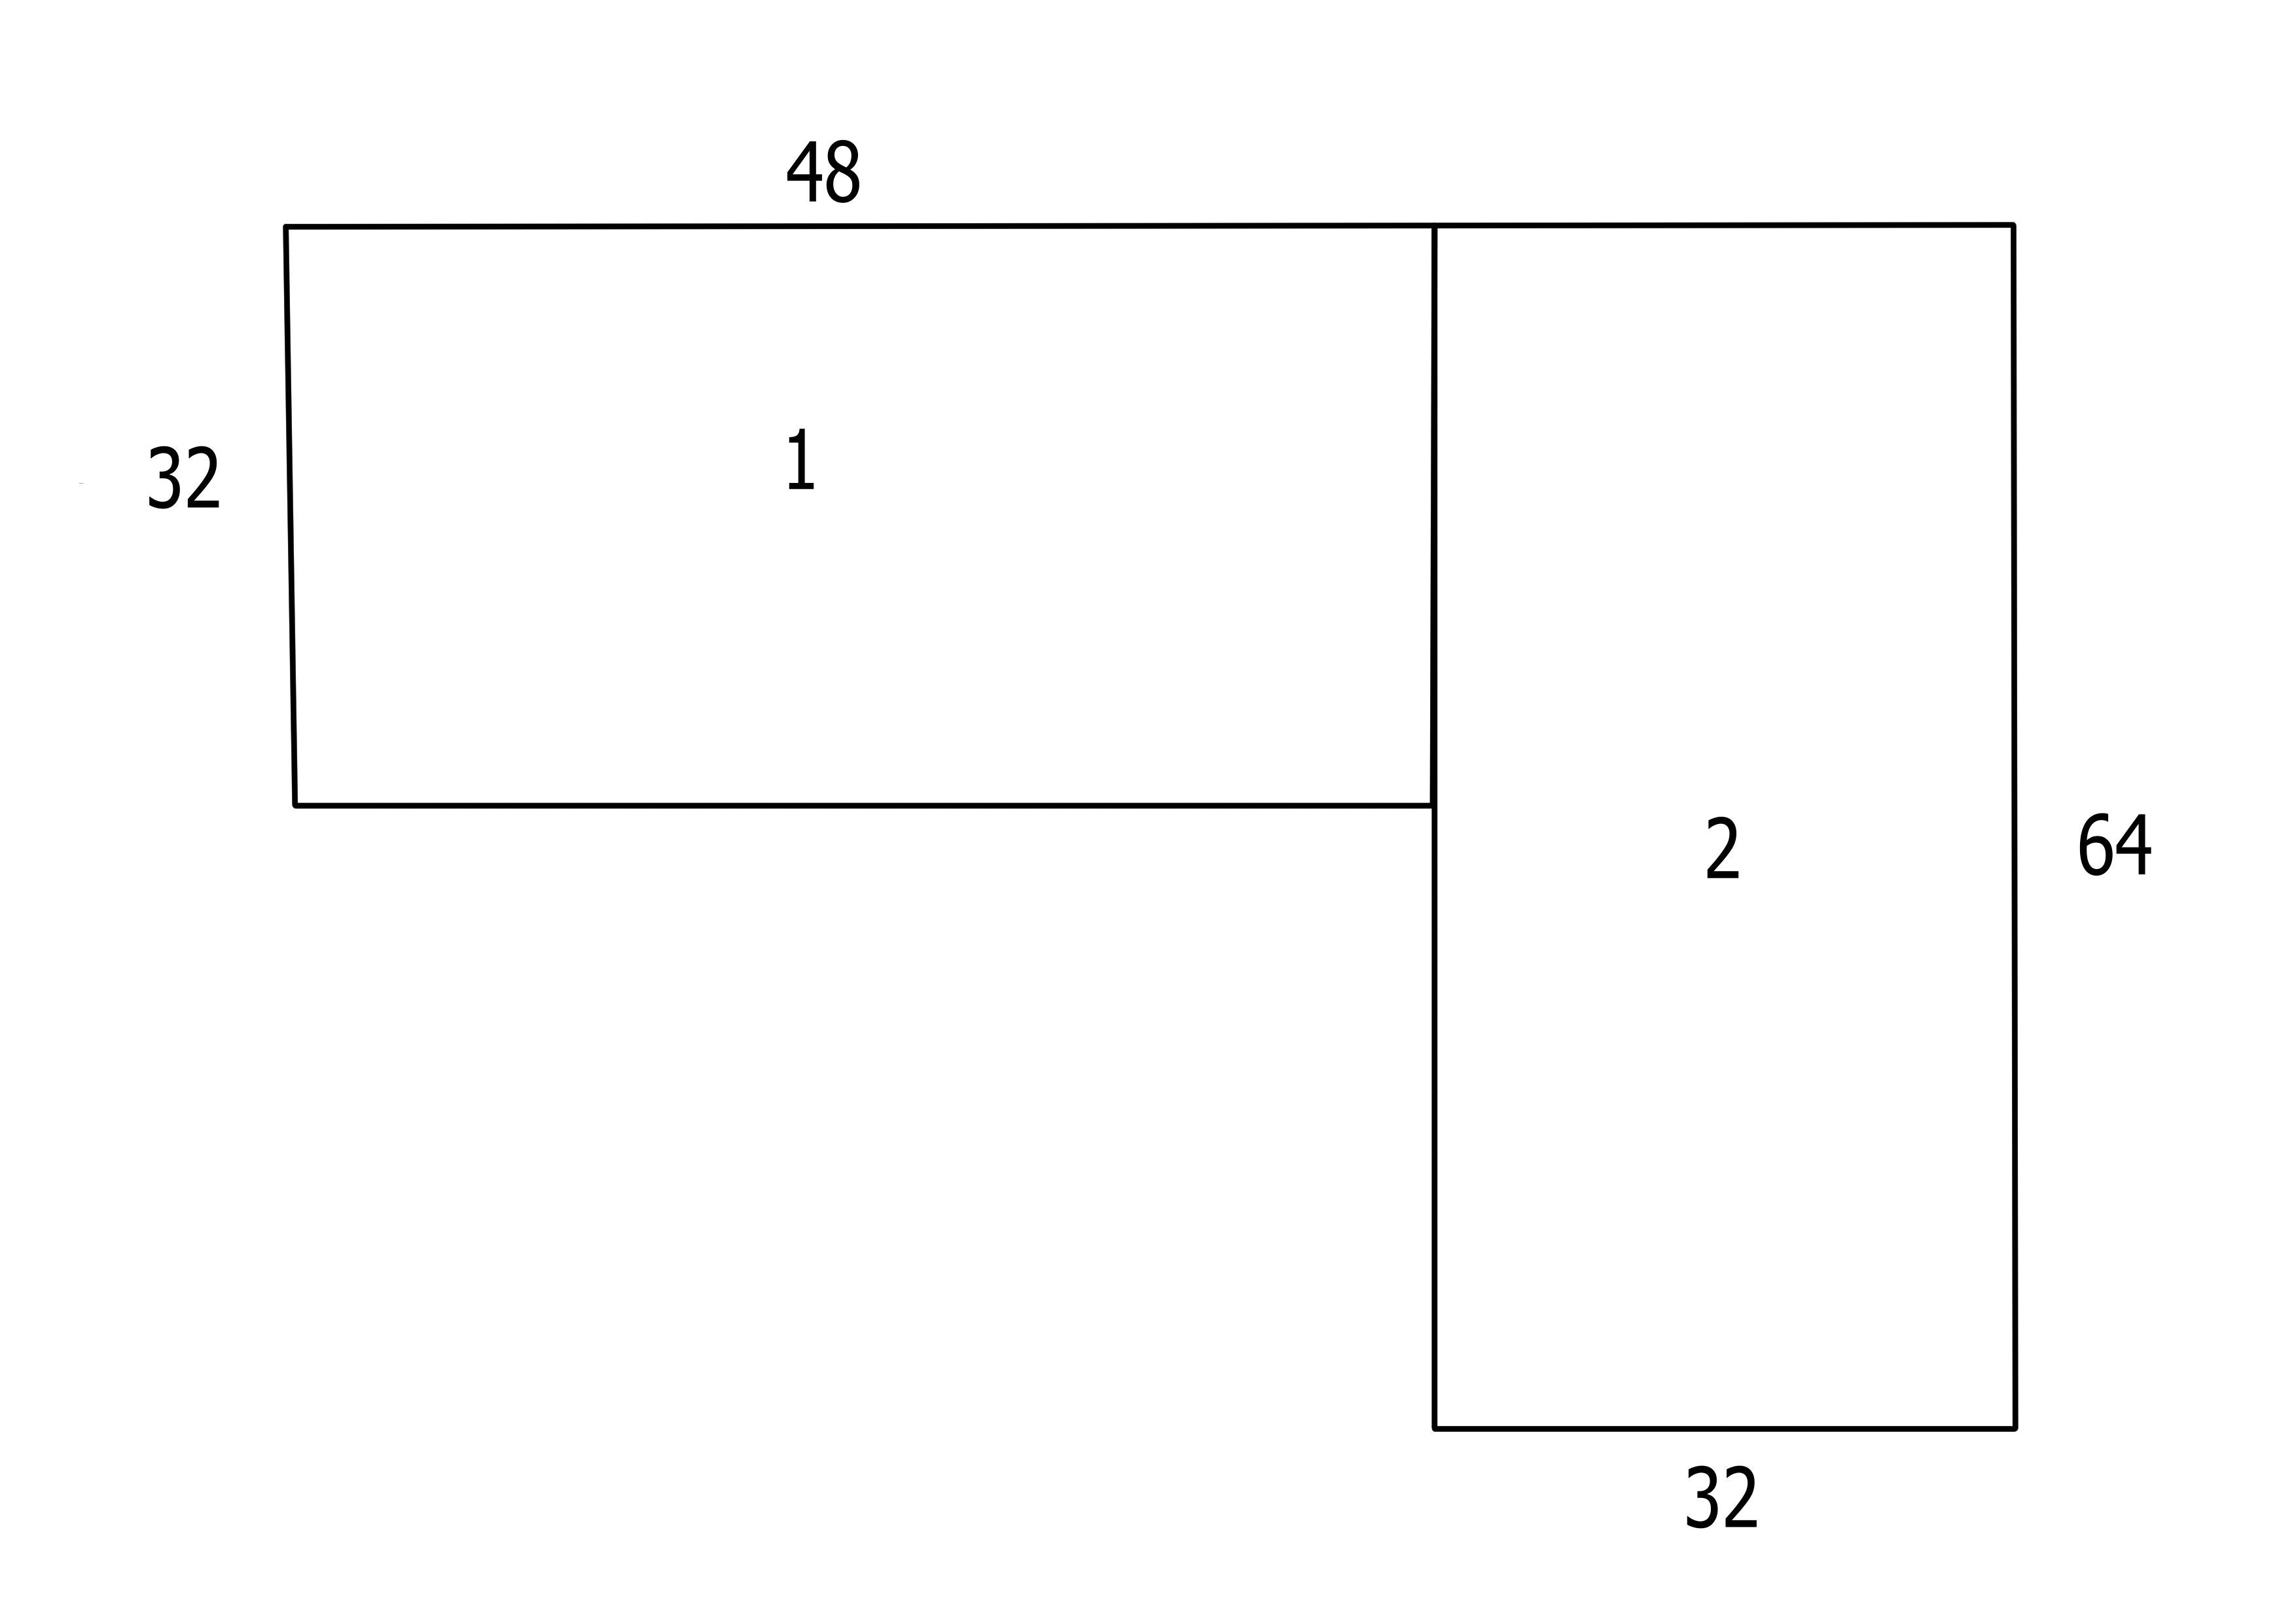
\includegraphics[width=.9\linewidth]{LShapeDomain1.jpeg}
\vspace{-20pt}
\caption{The Domain Decomposition}
\end{figure}

The decomposition of the L-shape is shown above and so for the first domain the code uses the given boundary conditions for the north, south and west boundaries and an average of the top halves of the 48th and 49th column on the east.

To verify the error and reflection free passing of an initial condition through the interface we compare the solution to one which is computed on a rectangle covering the whole L-shaped domain. Table (\ref{tab1}) details the conditions and results of the test with an initial condition of zeros except from a rectangle of ones from $x = 16$ to $32$, $y = 48$ to $52$ run for 50 time steps of $0.00667$.

\newpage

\begin{table}[h]

  \begin{center}
    \begin{tabular}{|l r|}
	\hline
	Variable & Value \\    
    \hline
    $a_x$ & 1 \\
    $a_y$ & 0.1\\
    Error & 4.2067e-16\\
    \hline
    \end{tabular}
  \end{center}
  \vspace{-10pt}
  \caption{Results of test}
 \label{tab1}
\end{table}

The results show that the difference in the two solutions is less than the accuracy of Matlab. This shows that our algorithm is error- and reflection-free across the interface between the decomposed domains. The plots given below show the initial condition for the test and also the solution at the end of the test. The second plot shows the smooth transition between domains as there are no obvious jumps.

\begin{figure}[h] 
\begin{minipage}{0.5\textwidth}
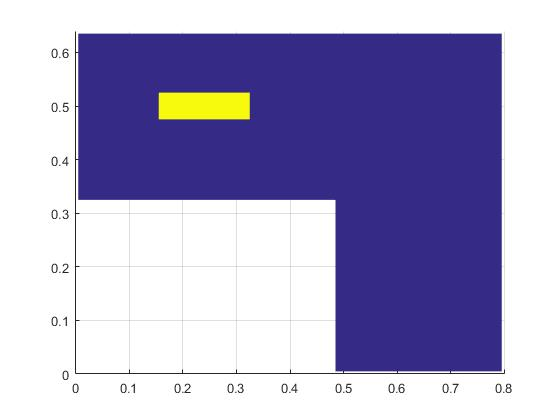
\includegraphics[width=1.1\linewidth]{Advec1.jpg}
\end{minipage}
\begin{minipage}{0.5\textwidth}
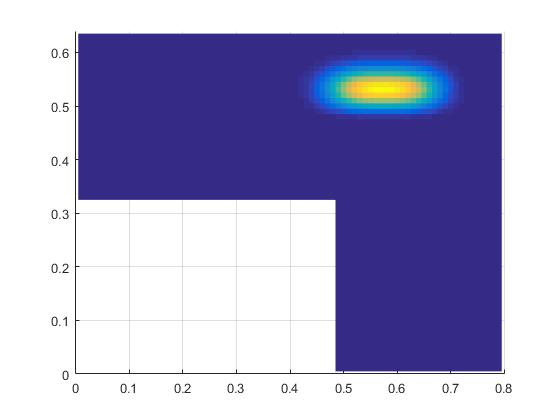
\includegraphics[width=1.1\linewidth]{Advec2.jpg}
\end{minipage}

\caption{Initial Condition and Final Plot of the Test}
\end{figure}


\newpage
%----------------------------------------------------------------------------------
\section{Diffusion}
%----------------------------------------------------------------------------------

The two-dimensional diffusion equation takes the form given in equation (\ref{diff.eqn}) and the question imposes inhomogeneous Dirichlet boundary conditions. $D$ controls the rate at which the solution diffuses.

\begin{equation}\label{diff.eqn}
\frac{\partial q}{\partial t} = D\left(\frac{\partial ^2 q}{\partial x^2} + \frac{\partial^2 q}{\partial y^2}\right)
\end{equation}

The L-shape domain is decomposed into two overlapping rectangles in order for the information to be passed from one to the other. The decomposition is given below in  figure (\ref{diff.decomp}). Using a new script, `DiffusionSolve.m' is called successively on each domain updating the boundary conditions at the overlap region boundaries as specified by the multiplicative alternating Schwarz algorithm. The code uses a while loop to run the alternating Schwarz until difference in solution between the two domains is below a specified tolerance.

	`DiffusionSolve.m' uses the multigrid method to solve the diffusion equation, which means A,R and P must be given. Fortunately both decomposed domains have the same dimensions and so as diffusion is orientation-less, transposing one of the domains means only one set of A,R and P need to be specified. A,R and P are given such that a Dirichlet condition is specified on the boundaries and A is adjusted to fit the given equation. 

\begin{figure}[h]
\vspace{-10pt}
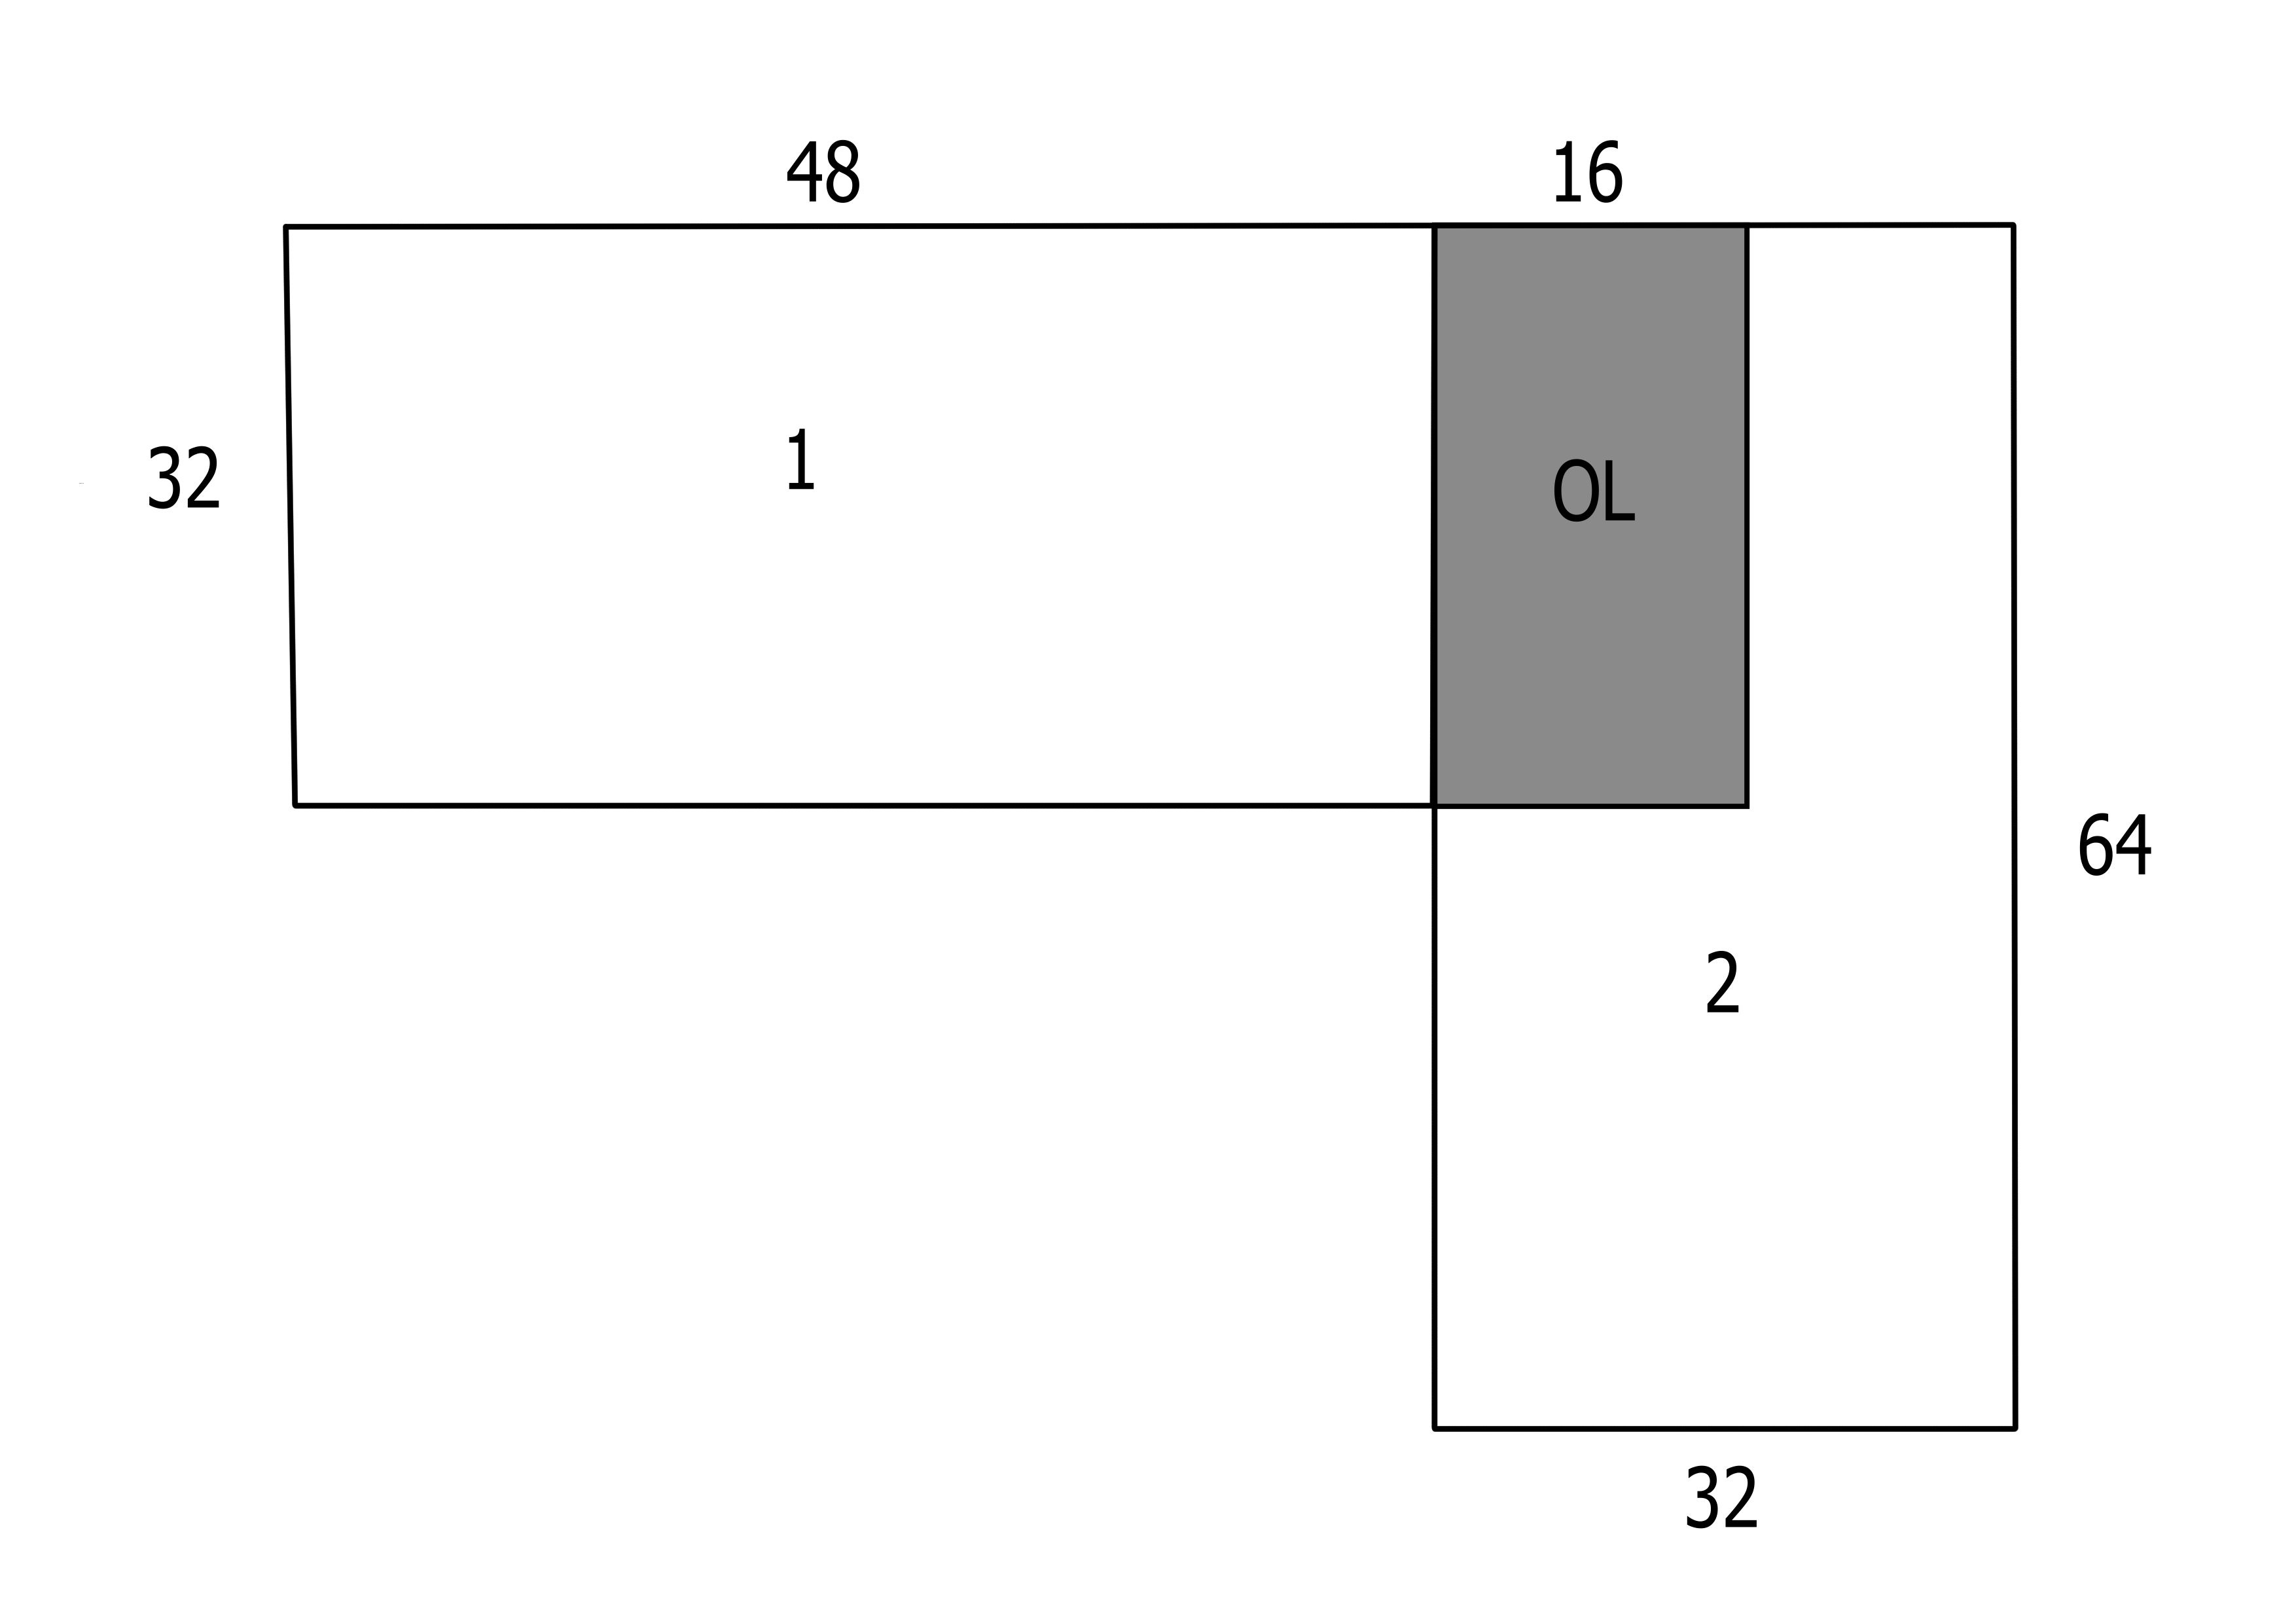
\includegraphics[width=.9\linewidth]{LShapeDomain2.jpeg}
\vspace{-20pt}
\caption{The Domain Decomposition for Diffusion}
\label{diff.decomp}
\end{figure}

To verify the numerical solution, we monitor the residual on the interface having selected a $D$ of $1/500$ (which corresponds to a Reynolds number of $500$) and final time of $1$ second, meaning $150$ time steps of size $0.01/1.5$. The boundary conditions were given as one on the north boundary and zero elsewhere. The plots created at the end of running the script can be found below in figure (\ref{diff.solplot}) and figure (\ref{diff.resplot}) is plot showing the decrease in the maximum difference between the solutions on the decomposed regions at each full iteration of the alternating Schwarz for the final time step.


\begin{figure}[h] 
\begin{minipage}{0.5\textwidth}
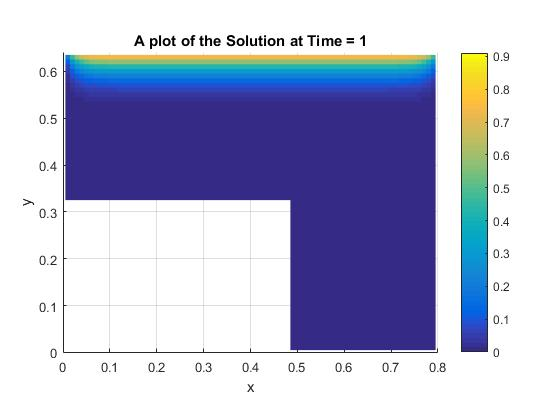
\includegraphics[width=1.1\linewidth]{Diff1.jpg}
\end{minipage}
\begin{minipage}{0.5\textwidth}
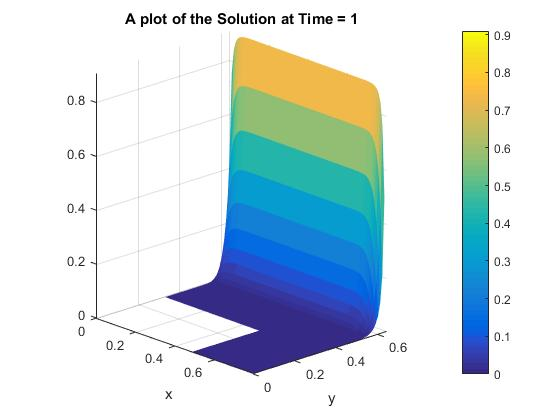
\includegraphics[width=1.1\linewidth]{Diff2.jpg}
\end{minipage}
\caption{The Solution at the end of the Test}
\label{diff.solplot}
\end{figure}

\begin{figure}[h] 
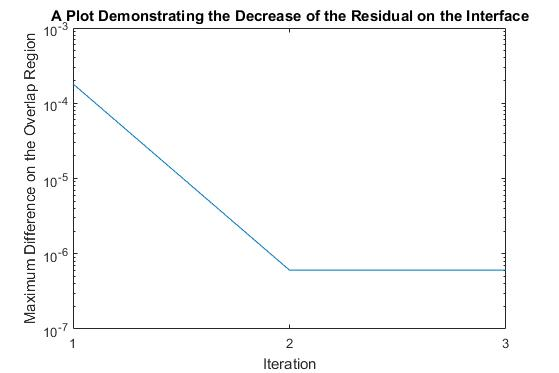
\includegraphics[width=.9\linewidth]{DiffRes1.jpg}
\caption{}
\label{diff.resplot}
\end{figure}

The plot above shows that after only two full iterations we reach the limit of accuracy that this method can achieve with machine error. Table (\ref{diff.table}) also shows this very clearly and the fast rate which is achieved.

\begin{table}[h]
  \begin{center}
    \begin{tabular}{|l|rr|}
	\hline
	Iteration & Error & Rate \\  
    \hline
    1 & 0.000180977	& - \\
    2 & 6.04982e-07 & 299.145 \\
    3 & 6.04982e-07 & 1\\
    \hline
    \end{tabular}
  \end{center}
  \vspace{-10pt}
  \caption{Results of test}
  \label{diff.table}
\end{table}
\newpage
This test demonstrates that my code is running as expected and the solution plots coincide with our intuition of diffusion. After this test I included a condition to stop the while loop when the rate of converges has decreased significantly, this means that time is not wasted running the alternating Schwarz when very little increase in accuracy can be achieved.


%----------------------------------------------------------------------------------
\section{Poisson}
%----------------------------------------------------------------------------------

The Poisson equation is an eliptic equation and unlike the first two, does not depend on time. For this section the boundary conditions around the L-shaped domain are homogeneous Neumann boundary conditions and the governing equation is the Poisson equation given below.

\begin{equation}
\frac{\partial^2 q}{\partial x^2} + \frac{\partial^2 q}{\partial x^2} = f\left(x,y\right)
\end{equation} 

Again the overlap region is used and the two decomposed domains are as in the diffusion section. However for this problem we have Neumann boundary conditions on the boundary of the L-shape and Dirichlet on the boundary of the overlap region. This means that A,P and R must be changed to account for the different types of boundary condition. For P, I splice together sections of a Dirichlet P and a Neumann P in order to get Dirichlet and Neumann on the same side of the rectangle and introduce a second set of A, P and R for the second rectangle. For A, I adjust the matrix after it has been created for Neumann BC. The Poisson equation with full Neumann boundary conditions is underdetermined and so to ensure the uniqueness of the solution we impose a single Dirichlet point on the boundary.

The multiplicative alternating Schwarz algorithm is implemented in exactly the same way as before, looping until the solutions coincide.

\begin{figure}[h]
\vspace{-10pt}
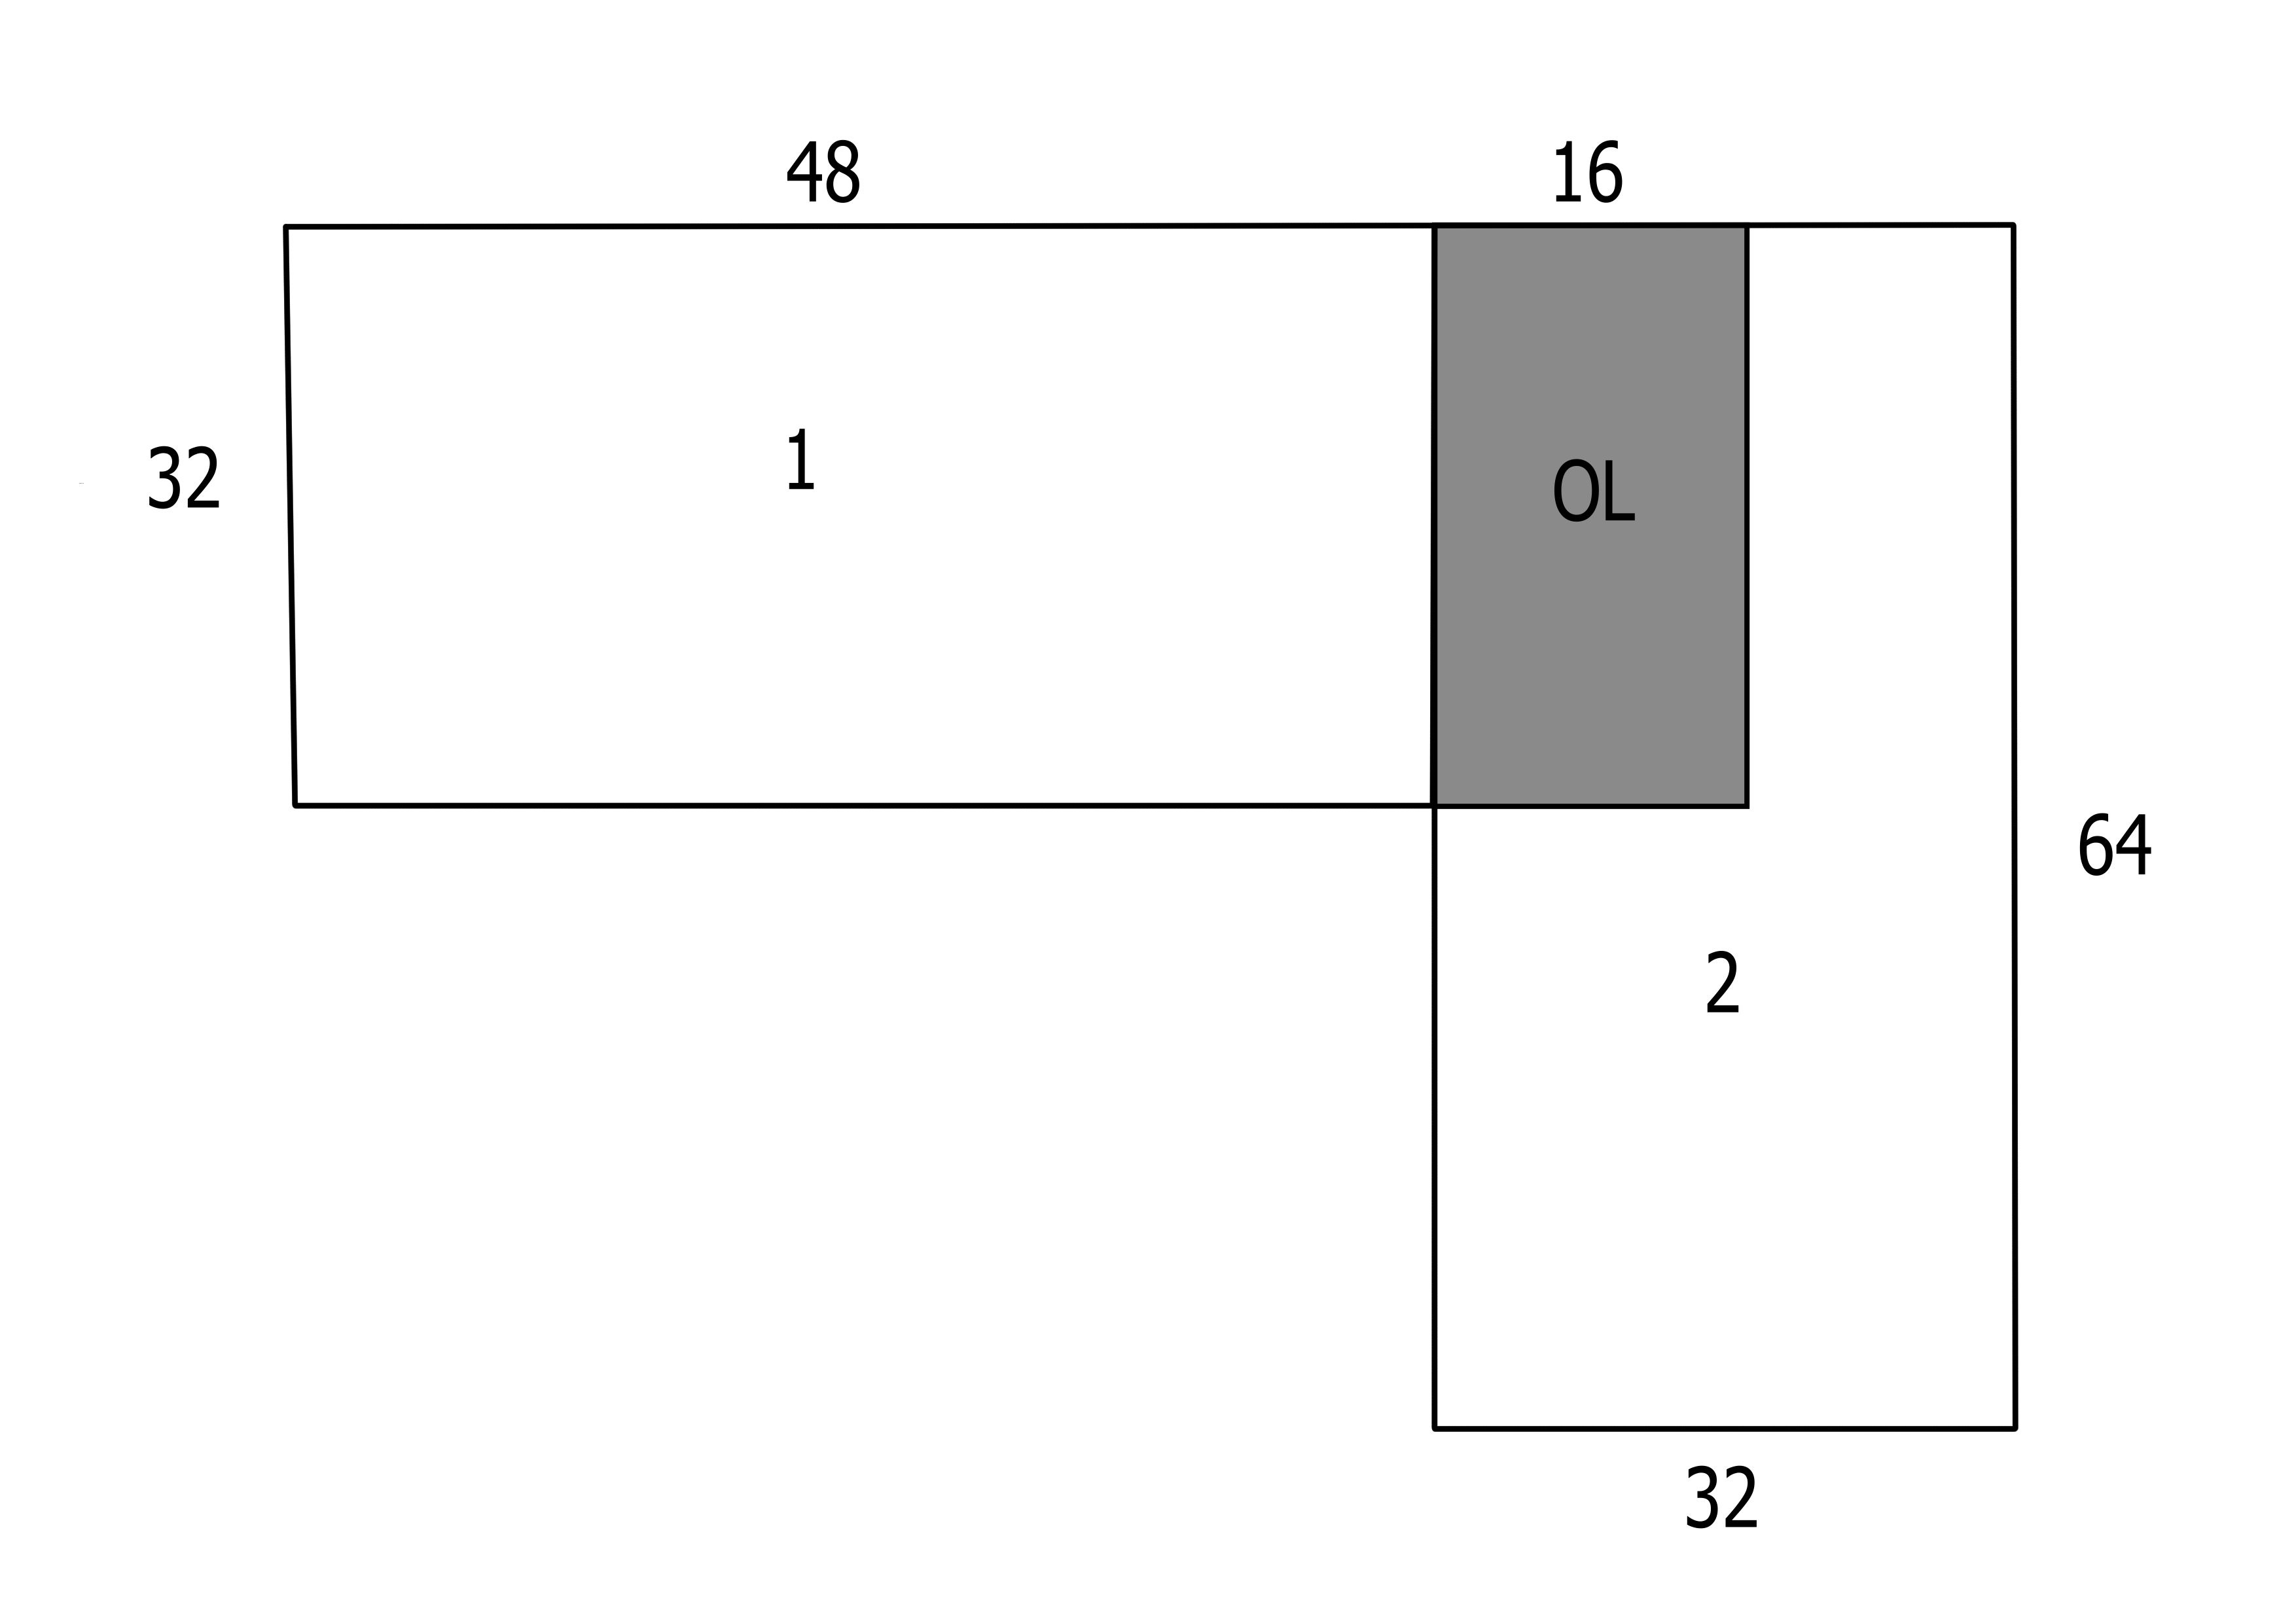
\includegraphics[width=.9\linewidth]{LShapeDomain2.jpeg}
\vspace{-20pt}
\caption{The Domain Decomposition for Poisson}
\label{poisson.decomp}
\end{figure}

\newpage

Again we verify the solution by monitoring the residual on the interface of a test problem. For this test we impose homogeous Neumann boundary conditions round the L-shaped domain (except for the single Dirichlet point), a right hand side in the Poisson equation of 1 and initial guess of zeros. Plots of the numerical solution are given in figure (\ref{poisson.solplot}), the spike is at the position of the imposed Dirichlet point. 


\begin{figure}[h] 
\begin{minipage}{0.5\textwidth}
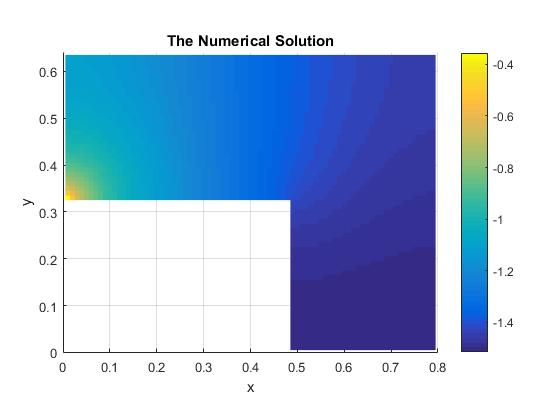
\includegraphics[width=1.1\linewidth]{Poisson1.jpg}
\end{minipage}
\begin{minipage}{0.5\textwidth}
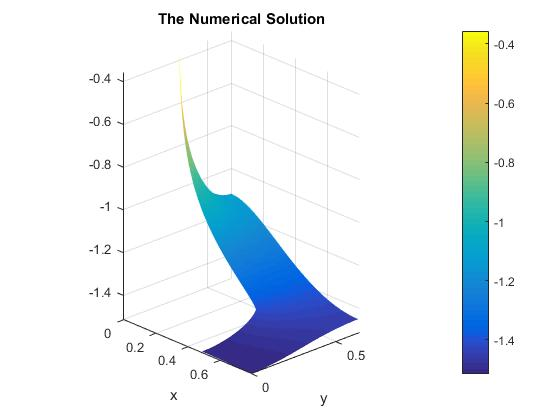
\includegraphics[width=1.1\linewidth]{Poisson2.jpg}
\end{minipage}
\caption{The solution at the end of the test 1}
\label{poisson.solplot}
\end{figure}

\newpage


\begin{figure}[h] 
\centering
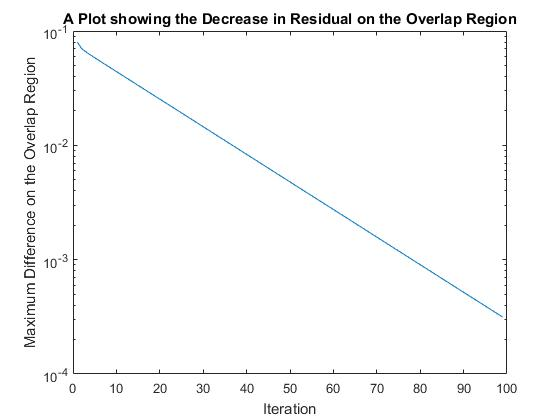
\includegraphics[width=.7\linewidth]{PoissonRes1.jpg}
\caption{Test 1}
\label{poisson.resplot}
\end{figure}

Above is a plot showing the steady decrease in the maximum difference of the two solutions on the overlap region. For all the tests, including those not included here, the rate of reduction settled to a constant $1.05714$ per iteration. This means that the initial guess of the solution is a big factor for number of iterations until the desired accuracy is achieved. 

To show this, the test was run again with a new initial condition of $-1.4$ everywhere. The original test resulted in a final maximum difference of 0.000314344 compared to 9.06051e-06 for the second test, the ratio of which is 34.6939. The plot for the second test is given below in figure (\ref{poisson.resplot2}).


\begin{figure}[h] 
\centering
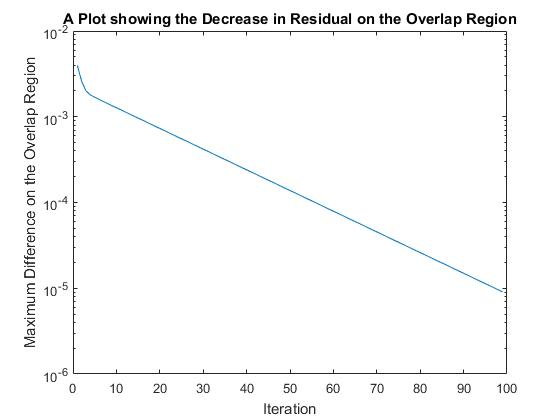
\includegraphics[width=.7\linewidth]{PoissonRes2.jpg}
\caption{Test 2}
\label{poisson.resplot2}
\end{figure}

\newpage
%----------------------------------------------------------------------------------
\section{Cavity Flow}
%----------------------------------------------------------------------------------

In this final section, the previous sections are put together to solve the incompressible Navier-Stokes equations (\ref{Cav.eqn1}, \ref{Cav.eqn2}) by operator splitting. The method begins with the advection part the result of which is used for the diffusion and finally the Poisson equation is used to correct the flow to take into account the pressure.

\begin{align} \label{Cav.eqn1}
\frac{\partial \bf{u}}{\partial t} + \bf{u} \nabla \bf{u} &= -\nabla p + \frac{1}{Re} \nabla^2\bf{u}\\ \label{Cav.eqn2}
\nabla \cdot \bf{u} &= 0
\end{align}

For this section most of the coding has been already completed in the previous sections, the script just needs to call the correct procedure for each part. However in order to solve for the pressure and to use the pressure to correct the flow the function `Diff.m' is called and this must be modified for the L-shaped domain. The modifications are simple: updating to account for the new boundary shape and sweeping only inside the L-shape.

I used my previous error calculating scripts to gain an understanding the error we could expect from the different parts. Diffusion has a lower bound for the error caused by the alternating Schwarz, to obtain the most accurate answer possible and computationally efficient the tolerances for the other scripts should just as accurate but not more. Through testing the error was found to be of the order 1e-7 and so I set 1e-7 to be my desired tolerance for my functions.  It is important to remember that the solution to the Poisson part is then used in the `Diff.m', this effectively multiplies the possible error by a factor of 1/dx (i.e. 100) thus we should set the tolerance on the pressure to be 1e-9.

However the Poisson script is the most computational expensive and for this error tolerance would take a very long time to run. To evade this issue, I used the fact that we are looking for a steady state solution, so small perturbation from this solution should revert back to the steady solution. This means that for low time steps we can reduce the tolerance on the pressure to decrease the computation time. The best way to do this is to restrict the alternating Schwarz to less iterations as when the solution is close to the steady state the error from the alternating Schwarz will decrease as the initial guess and final solution are much closer together. This also specifies the maximum computation time used for that the Poisson script for each time step.

The reduction in computation time is significant, with a max number of alternating Schwarz cycles set to 300 (so that the tolerance was always met) the script took 1545.709 seconds to reach a time step of 150 which is one second, 1533.044 of which were spent in `poissonSolve.m'. With a restriction to 5 alternating Schwarz cycles the time taken was 66.772, with 61.783 seconds in `poissonSolve.m'. Further details as to the loss of accuracy can be found in the table below (\ref{cav.tab1}).

\begin{table}[h] 
  \begin{center}
    \begin{tabular}{|rrr|}
	\hline
	Max Number of Cycles &  Time & Max Difference\\  
    \hline
	50 & 	593.689 & - \\
	5 & 	66.772 & 6.4830e-06 \\
    \hline
    \end{tabular}
  \end{center}
  \vspace{-10pt}
  \caption{Results of restricted Alternating Schwarz test}
  \label{cav.tab1}
\end{table}

From the brief error analysis, the error is approximately 1e-6. Now we can move on to studying the solution itself, starting with a plot of the velocity field (\ref{cav.vel1}) with Reynolds number 500.

\begin{figure}[h] 
\centering
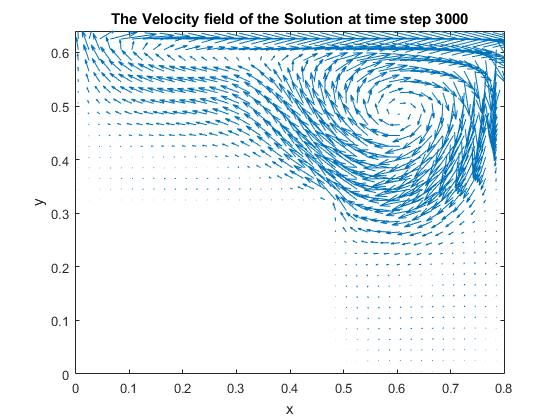
\includegraphics[width=1.1\linewidth]{CavityVel1.jpg}
\caption{Velocity field}
\label{cav.vel1}
\end{figure}

This plot clearly shows a main vortex centred at (0.605,0.49) spinning clockwise. We expect there to also be two smaller vortices at the ends of the L shape. The next two plots are an enlargement of those areas.

\newpage

\begin{figure}[h] 
\begin{minipage}{0.5\textwidth}
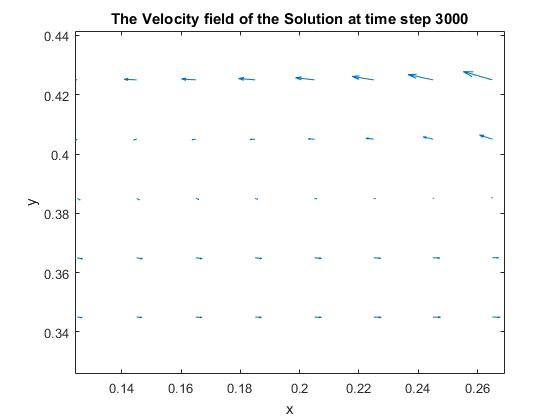
\includegraphics[width=1.1\linewidth]{CavityVel2.jpg}
\end{minipage}
\begin{minipage}{0.5\textwidth}
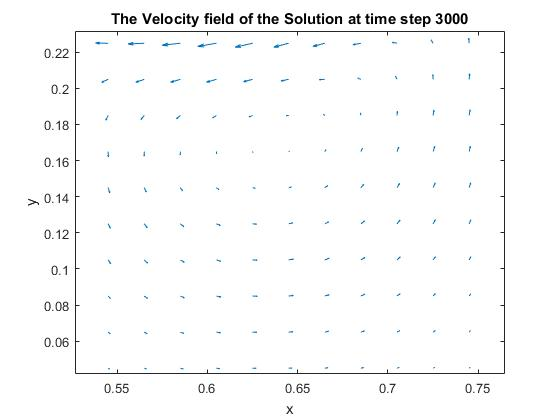
\includegraphics[width=1.1\linewidth]{CavityVel3.jpg}
\end{minipage}
\caption{Enlarged Sections}
\label{cav.vel2}
\end{figure}

Indeed the figure shows that two more vertices exist, one centred about (0.195,0.39) spinning anti-clockwise in an oval shape and the other centred at (0.64,0.17) spinning anti-clockwise too. Below are two plots of the vorticity of the solution. The one on the right has had it's colourmap clipped.


\begin{figure}[h] 
\begin{minipage}{0.5\textwidth}
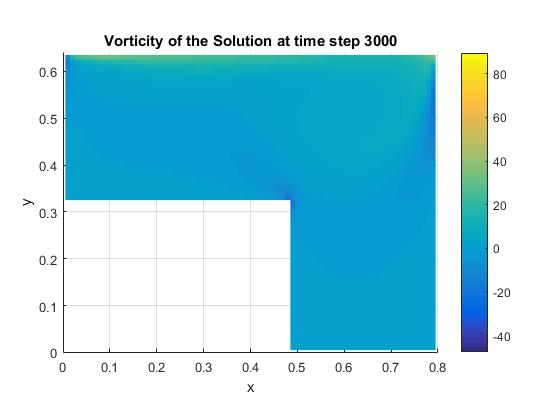
\includegraphics[width=1.1\linewidth]{CavityVort1.jpg}
\end{minipage}
\begin{minipage}{0.5\textwidth}
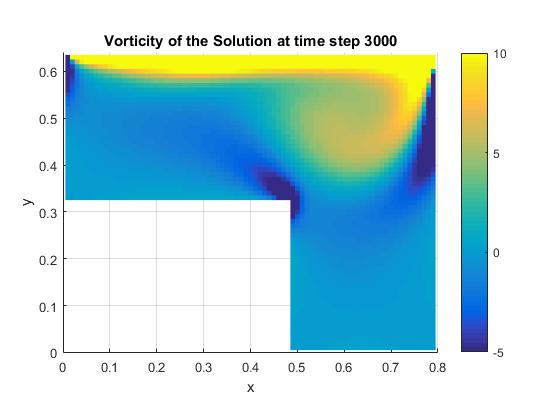
\includegraphics[width=1.1\linewidth]{CavityVort2.jpg}
\end{minipage}
\caption{Vorticity}
\label{cav.vort}
\end{figure}

Finally for this Reynolds number there is a plot of the max change in solution between consecutive time steps (\ref{cav.res1}). The plot shows an almost linear relationship with an average reduction in the max change of 1.0093 at each time step. The final values were 3.86862e-10 for u and 3.64871e-10 for v. This implies that the solution is close to a steady state of the numerical system.

\newpage

\begin{figure}[h] 
\centering
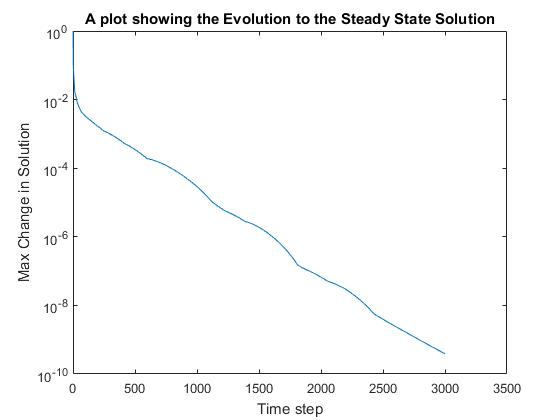
\includegraphics[width=.7\linewidth]{CavityRes1.jpg}
\caption{Change in Solution}
\label{cav.res1}
\end{figure}

Using the same code we can numerically solve many different fluid problem through adjusting the Reynolds number of the system. Following are the results of decreasing and increasing the Reynolds number about the 500 previously used.

\begin{figure}[h]
\begin{minipage}{0.6\textwidth}
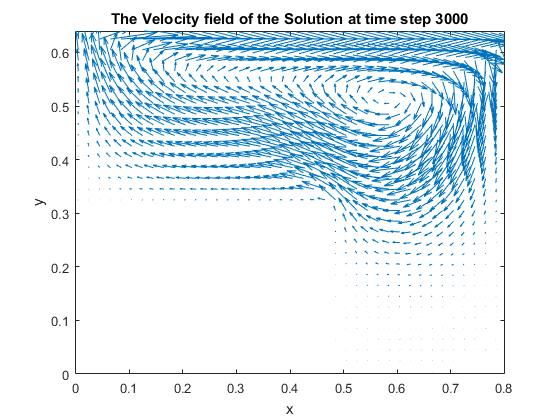
\includegraphics[width=1.1\linewidth]{Cavity100Vel1.jpg}
\end{minipage}
\begin{minipage}{0.3\textwidth}
If we reduce the Reynolds number to 100, this is equivalent to increasing the viscosity and as a result there is only one vortex.
\end{minipage}
\caption{Reynolds number = 100}
\label{cav.100vel1}
\end{figure}

\newpage

\begin{figure}[h]
\begin{minipage}{0.6\textwidth}
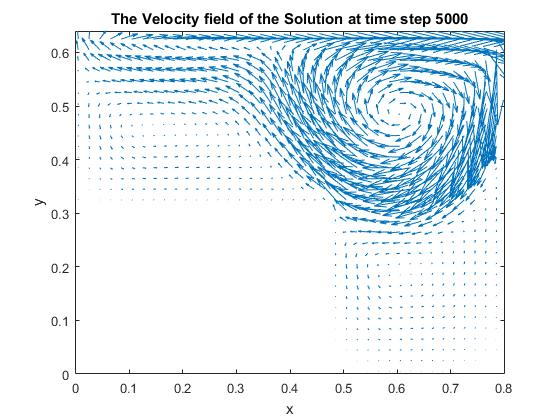
\includegraphics[width=1.1\linewidth]{Cavity2000Vel1.jpg}
\end{minipage}
\begin{minipage}{0.3\textwidth}
If we increase the Reynolds number to 2000, this is equivalent to reducing the viscosity and as a result the vortices become more pronounced.
\end{minipage}
\caption{Reynolds number = 2000}
\label{cav.2000vel1}
\end{figure}

In conclusion, the cravity flow code for a rectanglar domain has been successfully extended to an L shape domain. Only a small number of the possible problems on the L shape domain have been studied. The boundary and initial conditions could be changed to produce a variety of results and systems. The techniques use here also apply to adding more rectangular domains and so many different domains can be constructed, although I would recommend restructuring the code and the use of classes for easier domain decomposion.



\newpage
%----------------------------------------------------------------------------------
\begin{appendices}
%----------------------------------------------------------------------------------

\section*{Matlab Code}

%\lstinputlisting{DriverMGVRobin.m}
\lstinputlisting{CavityFlow/SemiLagrAdvectModified.m}
\lstinputlisting{CavityFlow/SemiLagrAdvectMain.m}
\lstinputlisting{SemiLagrAdvect/Question1Driver.m}

\lstinputlisting{Diffusion/DiffusionSolveModified.m}
\lstinputlisting{Diffusion/DiffusionSolveMain.m}
\lstinputlisting{Diffusion/Question2Driver.m}

\lstinputlisting{Poisson/GetAp.m}
\lstinputlisting{Poisson/GetRPp.m}
\lstinputlisting{Poisson/poissonSolve.m}
\lstinputlisting{Poisson/poissonSolveMain.m}


\lstinputlisting{CavityFlow/Diff2.m}
\lstinputlisting{CavityFlow/Question4Driver.m}

\end{appendices}
%----------------------------------------------------------------------------------


\begin{thebibliography}{9}


\bibitem{Code}
Prof. Peter Schmid provided a Matlab scripts containing the cavity flow code and its components, that was adapted and used in this project.

\end{thebibliography}



\end{document}
